\documentclass{IEEEcsmag}

\usepackage[colorlinks,urlcolor=blue,linkcolor=blue,citecolor=blue]{hyperref}

\usepackage{tabularx}
\usepackage{upmath}
\usepackage{amssymb}
\usepackage{amsmath}
\usepackage{array}
\usepackage{arydshln}
\usepackage{listings, multicol}
\usepackage{filecontents}
\usepackage{parcolumns}
\usepackage{booktabs}


\newcolumntype{P}[1]{>{\centering\arraybackslash}p{#1}}

\jvol{XX}
\jnum{XX}
\paper{8}
\jmonth{May/June}
\jname{Computing in Science and Engineering}
\pubyear{2021}
\newtheorem{theorem}{Theorem}
\newtheorem{lemma}{Lemma}

\setcounter{secnumdepth}{0}

\lstset{language=Python, basicstyle=\ttfamily\footnotesize}

\begin{filecontents*}{loop_fusion.py}
import numba
import numpy as np

# optionally the decorator can take
# the option nopython=True, which
# disallows Numba from running in
# object mode
@numba.jit
def loop_fusion(a):
    """
    An example of loop fusion, an
    optimization that Numba is able
    to perform on a user's behalf.
    When it recognizes that they are
    operating similarly on a single
    data structure
    """
    for i in range(10):
        a[i] += 1

    for i in range(10):
        a[i] *= 5

    return a
\end{filecontents*}

\begin{filecontents*}{nested_function.py}
import numpy as np
import numba
import numba.core
import numba.typed


# Dictionary instance created at runtime
results = numba.typed.Dict.empty(
    key_type=numba.core.types.unicode_type,
    value_type=numba.core.types.float64[:]
)

@numba.njit
def nested(input, results):
    # This function expects a
    # typed dictionary as an
    # argument to store results

    def step1(a):
        # first step of algorithm
        # store results in dictionary
        ...

    def step2(a):
        # second step of algorithm
        # store results in dictionary
        ...

    return results

\end{filecontents*}

\begin{filecontents*}{parallel_multithreading.py}
import numba
import numpy as np

@numba.njit(cache=True, parallel=True)
def multithreading(a):

	for i in numba.prange(10):
		a[i] *= 10

\end{filecontents*}


\begin{document}

\sptitle{Department: Head}
\editor{Editor: Name, xxxx@email}

\title{PyExaFMM: an exercise in designing high-performance software with Python and Numba}

\author{S. Kailasa}
\affil{Department of Mathematics, University College London}

\author{T. Wang}
\affil{Department of Mechanical and Aerospace Engineering, The George Washington University}

\author{\text{L}. A. Barba}
\affil{Department of Mechanical and Aerospace Engineering, The George Washington University}

\author{T. Betcke}
\affil{Department of Mathematics, University College London}

\markboth{Department Head}{Paper title}

\begin{abstract}
    Numba is a game changing compiler for high performance computing with Python. The machine code it produces runs outside of the single-threaded Python interpreter, and can therefore fully utilize the resources of modern CPUs. This means support for parallel multithreading and auto vectorization if available, just like in a compiled language such as C++ or Fortran. In this paper document our experience with Numba as we developed PyExaFMM, a fully multithreaded Numba implementation of the Fast Multipole Method, an algorithm with a a non-linear data structure and a significant amount of data organization. We find that designing highly performant Numba code for complex algorithms can be as challenging as writing in a compiled language.
\end{abstract}

\maketitle
\chapterinitial{Python}\footnote{We use `Python' to refer to CPython, the popular C language implementation of Python, which is dominant in computational science.}, is designed for memory safety and programmer productivity. Its simplicity allows Computational Scientists to spend more time exploring the science, and less time being confused by strange software quirks, memory errors, and the nightmare of incompatible dependencies, which conspire to drain productivity in lower level languages.

The catch is that code is run through an interpreter and restricted to a single thread via a software construction called the Global Interpreter Lock [GIL]. Libraries for high performance computational science have traditionally bypassed the issue of the GIL by using Python's C interface to call extensions built in C or other compiled languages which can be multithreaded or compiled to target special hardware features. Popular examples of this approach include Numpy and SciPy, which have together helped to propel Python's popularity in computational science by providing high performance data structures for numerical data as well as interfaces for compiled implementations of common algorithms from numerical linear algebra, to differential equation solvers and machine learning.

As the actual number-crunching happens outside of the interpreter, the GIL only becomes a bottleneck to performance if a program must repeatedly pass control between the interpreter and non-Python code. This is most often an issue when an optimized compiled language implementation of your desired algorithm doesn't exist in the Python Open Source, or if it requires a lot of data organization to form the input for an optimized Numpy or SciPy code, which must unavoidably take place within the interpreter. Previously, an unlucky developer would have been forced to write a compiled implementation to tackle these issues themselves and connect it to their Python package, relegating Python's role to an interface. However, not all Computational Scientists have the necessary software skills or research interest in developing and maintaining complex codebases that couple multiple languages.

This is the context in which Numba was introduced \cite{Lam2015}. It is a compiler that specifically targets and optimizes Python code written with Numpy's $n$-dimensional array, or `ndarray', data structure. Its power comes from the ability to generate multithreaded architecture optimized compiled code while \textit{only writing Python}. The promise of Numba is the ability to develop applications with speed that can rival C++ or Fortran, while retaining the simplicity and productivity of working in Python. We put this promise to the test by developing PyExaFMM\footnote{https://github.com/exafmm/pyexafmm}, an implementation of the Kernel Independent Particle Fast Multipole Method [FMM] \cite{Ying2004,Greengard1987}, in three dimensions. Efficient implementations of this algorithm are complicated by its reliance on a tree data structure and a series of operations which each require significant data organization and careful memory allocation. These features made PyExaFMM an excellent test case to see whether Numba could free us as Computational Scientists from the complexities of compiled languages.

We begin with an overview of Numba's design and its major pitfalls. After introducing the data structures and computations involved in the FMM, we provide an overview of how we implemented our software's data structures, algorithms and application programming interface [API] to optimally use Numba.

\section{NUMBA}

Numba targets code written using ndarrays, which are homogeneously typed and stored contiguously in memory. This means that adjacent elements are stored in adjacent memory locations. When loading data from a given memory location, modern CPUs cache data from adjacent locations. Therefore, algorithms which iterate sequentially over arrays benefit from lower memory loading latencies, as the CPU's cache is likely to contain the next element being operated on. This behavior is called \textit{cache locality}, and contrasts with Python lists, where subsequent elements need not be stored in adjacent memory locations and are found by following trails of pointers. This is called \textit{indirection}, and means that data stored in lists cannot take advantage of CPU caching. Ndarrays have fields describing their data's dimensionality, type, and layout, which Numba uses to generate machine code without any indirection. Instead it directly references the memory locations being referred to by Python code at runtime. This allows Numba to index into ndarrays with performance that can match compiled languages.

Numba is built with LLVM, a framework for building custom compilers, that provides an API to generate machine code for different hardware architectures such as CPUs and GPUs. LLVM is also able to analyze the code for hardware level optimizations, such as auto vectorization, and automatically apply them if they are available on the target hardware \cite{Lattner2004}.

From a programmer perspective using Numba naively doesn't involve a significant rewrite of code. Python functions are marked for compilation with a special decorator (see listings (\ref{code:loop_fusion}), (\ref{code:nested_function}) and (\ref{code:parallel_multithreading}) for example syntax).

Figure (\ref{fig:numba}) illustrates the program execution path when a Numba decorated function is called from the Python interpreter. We see that Numba doesn't replace the Python interpreter. If a marked function is called at runtime, program execution is handed to Numba's runtime which compiles the function on the fly s a type signature matching the input arguments. This is the origin of the term `just in time' [JIT] to describe such compilers.

The Numba runtime interacts with the Python interpreter dynamically, and control over program execution is passed back and forth between the two. There is a cost to this interaction from having to `unbox' Python objects into types compatible with the compiled machine code, and `box' the outputs of the compiled functions back into Python compatible objects. This process doesn't involve re-allocating memory, however pointers to memory locations have to be converted and placed in a type compatible with either Numba compiled code or Python.

\lstinputlisting[float=t, caption={An example of using Numba in a Python function operating on ndarrays.}\label{code:loop_fusion}]{loop_fusion.py}

\section{PITFALLS OF NUMBA}\label{sec:pitfalls}

Since its first release Numba has been extended to compile most functionality from the Numpy library, as well as the majority of Python's basic features and standard library modules\footnote{A full list of supported features for the current release can be found at: https://numba.pydata.org/numba\-doc/dev/reference/pysupported.html}. However, if Numba isn't able to find a suitable Numba type for each Python type in a decorated function, or it sees a Python feature it doesn't yet support, it runs in `object mode', handling all unknown quantities as generic Python objects. To ensure a seamless experience Numba does this without reporting it to the user. However, as object mode often no faster than ordinary vanilla Python, it puts the burden on the programmer to understand when and where Numba works and the principles of its implementation to adapt their implementation accordingly. As Numba influences the way Python is written it's more akin to a programming framework rather than just a compiler.

Additionally, not every supported feature behaves in a way a Python programmer would expect which has an impact on program design. An example of this arises when using Python dictionaries, which are central to Python, but are only partially supported by Numba. As they are untyped, and can have any Python objects as members, they don't neatly fit into a Numba compatible type. Programmers can declare a Numba compatible `typed dictionary', where the keys and values are constrained to Numba compatible types, and pass it to a Numba decorated function at low cost. However, using a Numba dictionary from the Python interpreter is \textit{always slower} than an ordinary Python dictionary due to the (un)boxing cost when getting and setting any item.

An example of Numba's framework-like behavior arises when implementing algorithms that share data, and have multiple logical steps as in listing (\ref{code:nested_function}). Numba's compiler doesn't distinguish between \lstinline{algorithm1} and \lstinline{algorithm2}, and both pay a cost to call subroutines defined outside of their function body, running in $308 \pm 1 \mu s$ and $306 \pm 1 \mu s$\footnote{Statistics calculated over seven trials}, respectively\footnote{All experiments are taken on an AMD Ryzen Threadripper 3970X 32-Core processor running Python 3.8.5 and Numba 0.53.0}. However, the nested function in \lstinline{algorithm3} is interpreted as a single function body by Numba, and runs in just $2.64 \pm 0.07 \mu s$. This an example of an \textit{inlining} optimization being taken by LLVM, and generalizes to less trivial examples. Mested functions have the tendency to grow long in Performant Numba code, in order to minimize the number of interactions between Numba and Python. However this makes them more difficult to unit test.

Therefore, performant Numba code can look quite un-Pythonic. Numba encourages fewer user created objects, performance critical sections written in terms of loops over simple array based data structures - reminiscent of C, and long nested functions. 

Though Numba is advertised as an easy way of injecting performance into your program via a simple decorator it has its own learning curve. Achieving performance requires a programmer to be somewhat familiar with the internals of its implementation (fig. (\ref{fig:numba})), and potentially have to radically change the design of their algorithms and data structures to avoid back and forth between the Numba runtime and the Python interpreter.

\begin{figure*}
    \centerline{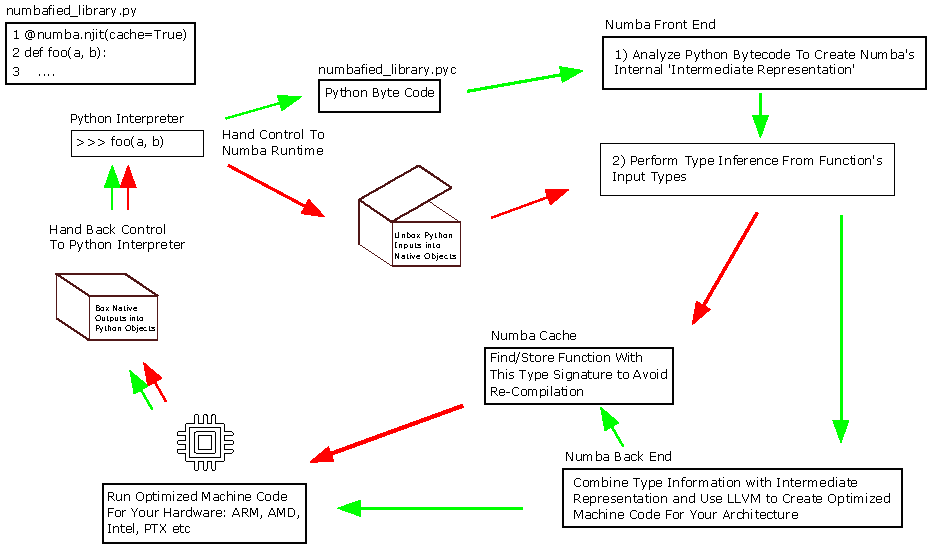
\includegraphics {figures/numba.pdf}}
    \caption{Simplified execution path when calling a Numba compiled function from the Python interpreter. The green path is only taken if the function hasn't been called before. The red path is taken if a compiled version with the correct type signature already exists in the Numba cache.}
    \label{fig:numba}
\end{figure*}

\lstinputlisting[caption={Three ways of writing a trivial algorithm that passes around a vector, while performing some computations.}\label{code:nested_function}]{nested_function.py}

\section{THE FAST MULTIPOLE METHOD}

The particle FMM is an approximation algorithm for $N$-body problems, in which $N$ source particles interact with $N$ target particles \cite{Greengard1987}. Consider the calculation of electrostatic potentials in 3D, which we use as our reference problem. A set of $N$ charged particles at positions $x_i$. The potential, $\phi_j$, at a given target particle at $x_j$ due to all other particles, excluding self interaction, can be written as.

\begin{equation}
    \phi_j = \sum_{i=1, i \neq j}^{N} \frac{q_i}{4 \pi| x_i-x_j |}
    \label{eq:laplace_kernel}
\end{equation}

where $\frac{1}{4 \pi| x_i-x_j|}$ is called the kernel, or the Green's function, and $q_i$ is the charge at $x_i$. The naive computation over all particles is $O(N^2)$, however the FMM compresses groups of interactions far away from a given particle using \textit{expansions}, reducing the overall complexity to $O(N)$. Expansions approximate charge contained within subregions of the octree, and can be truncated with to a desired accuracy, defined by a parameter, $p$, called the expansion order. The value of $p$ is equal to the number of digits of precision of the final solution. Problems with this structure appear with such frequency in science and engineering that the FMM has been described as one of the ten most important algorithms of the twentieth century \cite{Cipra2000}.

The algorithm relies on a hierarchical octree data structure to discretize the problem domain in 3D (see fig. 1 \cite{Sundar2007}) and consists of eight operators: P2M, P2L, M2M, M2L, L2L, L2P, M2P and the `near field', applied \textit{once} to each applicable node over the course of two consecutive traversals of the octree (bottom-up and then top-down). The operators define interactions between a given `target' node, and potentially multiple `source' nodes from the octree. They are read as `X to Y', where `P' stands for particle(s), `M' for \textit{multipole expansion} and `L' for \textit{local expansion}. The direct calculation of (\ref{eq:laplace_kernel}) is referred to as the P2P operator, and is used as a subroutine during the calculation of the other operators. The Kernel Independent FMM [KIFMM] \cite{Ying2004}, implemented by PyExaFMM, is a re-formulation of the FMM with a structure that favours parallelization. Indeed all of the operators can be decomposed into matrix-vector products, or multithreaded implementations of (\ref{eq:laplace_kernel}), which are easy to optimize for modern hardware architectures, and fit well with Numba's programming framework. We defer to the FMM literature for a more detailed discussion on the mathematical significance of these operators \cite{Ying2004,Greengard1987}.

\section{COMPUTATIONAL STRUCTURE OF FMM OPERATORS}

The computational complexities of KIFMM operators are defined by a user specified $n_{crit}$, which is the maximum allowed number of particles in a leaf node, $n_e$ and $n_c$ which are the numbers of quadrature points on the \textit{check} and \textit{equivalent} surfaces respectively (see sec. 3 \cite{Ying2004}). The parameters $n_e$ and $n_c$ are quadratically related to the expansion order, i.e. $n_e = 6(p-1)^2 + 2$ \cite{Ying2004}. Typical values for $n_{crit}$ used are $\sim 100$. Notice the depth of the octree is defined $n_{crit}$, and hence by the particle distribution.

The near field, P2M, P2L, M2P, and L2P operate independently over the leaf nodes. The M2L and L2L operate independently on all nodes at a given level, from level 2 to the leaf level, during the top-down traversal. The M2M is applied to each node during the bottom-up traversal.

All operators, except the M2L M2M and L2L, rely on the P2P. The inputs for the P2P are vectors for the source and target positions, and the source charges or expansion coefficients; the output is a vector of potentials.

The inputs to the M2L, M2P, P2L and near field operators are defined by `interaction lists' called the V, W, X and U lists respectively. These interaction lists define the nodes a target node interacts with when an operator is applied to it. We can restrict the size of these interaction lists by demanding that neighboring nodes at the leaf level are at most twice as large as each other \cite{Sundar2007}. Using this `balance condition', the V, X, W and U lists in 3D contain at most 189, 19, 148 and 60 nodes, respectively.

The near field operator applies the P2P between the charges contained in the target and the source particles of nodes in its U list, in $O(60 \cdot n_{crit}^2)$. The M2P applies the P2P between multipole expansion coefficients of source nodes in the target's W list and the charges it contains internally in $O(148 \cdot n_e \cdot n_{crit})$. Similarly, the L2P applies the P2P between a target's own local expansion coefficients and the charges it contains in $O(n_e \cdot n_{crit})$.

The P2L, P2M and M2L involve creating local and multipole expansions, and rely on a matrix vector product related to the number of source nodes being compressed, which for the P2L and M2L are defined by the size of the target node's interaction lists. These matrix vector products have complexities of the form $O(k \cdot n_e^2)$ where $k = |X| = 19$ for the P2L, $k = |V| = 189$ for the M2L, and $k = 1$ for the P2M. Additionally, the P2L and P2M have to calculate `check potentials' (see sec. 3 \cite{Ying2004}) which require $O(19 \cdot n_{crit} \cdot n_c)$ and $O(n_{crit} \cdot n_c)$ calculations respectively. The M2M and L2L operators both involve translating expansions between nodes their eight children, and rely on a matrix vector product of $O(n_e^2)$.

The structure of the FMM's operators expose natural parallelism. The P2P is embarrassingly parallel over each target. As are the M2L, M2P, P2L and near field operators over their interaction lists. The near field, L2P, M2P, P2L and P2M operators are also embarrassingly parallel over the leaf nodes, as are the M2L, M2M and L2L over the nodes at a given level.

\section{DATA ORIENTED DESIGN}

Data oriented design is about writing code that operates on data structures with simple memory layouts, such as arrays, in order to optimally take advantage of modern hardware features. The idea being that it is easier for programmers to optimize for cache locality and parallelization if the data structures are easier to map to the hardware.

This contrasts with object oriented design, where although code is organized around data the focus is on user created types or `objects', where memory layout is obfuscated by the potential complexity of an object, which can contain multiple attributes of different types. This makes it harder to write code that takes advantage of cache locality. Numba's focus on ndarrays strongly encourages data oriented design principles, which are reflected in the design of PyExaFMM's octrees as well as its API.

Octrees can either be `pointer based' \cite{Wang2021}, or `linear' \cite{Sundar2007}. A pointer based octree, as in uses objects to represent each node, with fields for a unique id, contained particles, associated expansion coefficients, potentials, and pointers to their parent and sibling nodes. This makes searching for neighbors and siblings easy, as one has to just follow pointers. The linear octree implemented by PyExaFMM represents nodes by a unique id stored in a 1D vector, all other data such as expansion coefficients, particle data, and calculated potentials, are also stored in 1D vectors. Data is looked up by creating indices to tie a node's unique id to the associated data. This is an example of how Numba can affect design decisions, and make software more complex, despite the data structures being simpler.

Figure (\ref{fig:design}) illustrates PyExaFMM's design. There is only a single Python object, `Fmm', which acts as the API. It initializes ndarrays for expansion coefficients and calculated potentials, and its methods interface with Numba compiled functions for the FMM operators and their associated data manipulation functions. When sharing data we prefer nested functions, however we keep the operator implementations separate from each other, which allows us to unit test them individually. This means that we must have at least one interaction between Numba and the Python interpreter to call the near field, P2M, L2P, M2P and P2L operators, $d-2$ interactions to call the  M2L and L2L operators, and $d$ interactions for the M2M operator where $d$ is the depth of the octree. The most performant implementation would be a single Numba routine that interacts with Python just once, however this would sacrifice other principles of clean software engineering such as modularity, and unit testing.

This structure has strong parallels with software designs that arise from traditional methods of achieving performance with Python by interfacing with a compiled language such as C or Fortran. The benefit of writing in Numba is that we can continue to write in Python. Though as seen above, performant Numba code may only be superficially Pythonic through its shared syntax.

% Larger figure
\begin{figure*}
    \centerline{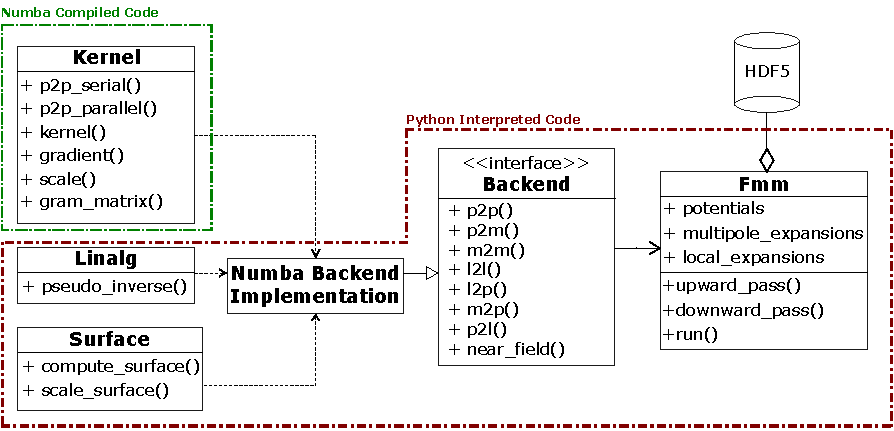
\includegraphics {figures/software.pdf}}
    \caption{Simplified UML model of all PyExaFMM components. Trees and other precomputed quantities are stored in a HDF5 database. The `Fmm' object acts as the user interface, all other components are modules consisting of methods on operating on arrays.}
    \label{fig:design}
\end{figure*}

\section{MULTITHREADING IN NUMBA}

Numba enables multithreading via a simple parallel for loop syntax (see listing (\ref{code:parallel_multithreading})) reminiscent of OpenMP. Internally Numba can use either OpenMP or Intel TBB to generate multithreaded code. We choose OpenMP for PyExaFMM, as it's more suited to functions in which each thread has an approximately similar workload. The threading library can be set via the \lstinline{NUMBA_THREADING_LAYER} environment variable.

Numerical libraries such as Numpy and SciPy implement many of their mathematical operations using multithreaded compiled libraries internally, such as OpenBLAS or IntelMKL. Numba compiled versions of these operations retains this internal multithreading. This leads to \textit{nested parallelism} when combined with a multithreaded region declared with Numba, as in listing (\ref{code:parallel_multithreading}). This is where a parallel region calls a function with another parallel region inside it. Threads created by the two functions are not coordinated by Numba, and this leads to \textit{oversubscription}, where the number of active threads exceeds the CPU's hardware capacity. Many threads are left idle while the CPU is forced to jump between threads operating on different data. This leads to broken cache locality, and hanging threads threads, stuck waiting for others to finish \cite{Malakhov2016}. We avoid this in PyExaFMM by explicitly setting Numpy operations to be single threaded, via the environment variable \lstinline{OMP_NUM_THREADS=1}, before starting our program. This ensures that the only threads created are those explicitly declared using Numba.

\lstinputlisting[float=t, caption={An example of parallel multithreading.}\label{code:parallel_multithreading}]{parallel_multithreading.py}

\section{PARALLELIZATION STRATEGIES FOR FMM OPERATORS}

In order to achieve an appropriate load balance such that the cost of creating and coordinating a thread did not exceed the cost of the computation it was responsible for, we avoided parallelizing over interaction lists.

The P2P, P2M, P2L, M2P, L2P and near field operators all rely on the P2P operator and are parallelized over their targets, the leaf nodes.

For the L2P operator we encourage cache locality for the P2P step, and keep the data structures passed to Numba as simple as possible, by allocating 1D vectors for the source positions, target positions and the source expansion coefficients, such that all the data required to apply an operator to single target node is adjacent in memory. By storing a vector of `index pointers', that bookend the data corresponding to each target in these 1D vectors, we can form parallel for loops over each target to compute the P2P that encourages cache-locality in the CPU. In order to to this, we have to first iterate through the target nodes, and lookup the associated data to fill the cache local vectors. Figure (\ref{fig:l2p_cache}) shows the speedup achieved with this strategy increases moderately with the number of calculations in each parallel thread.


 % Smaller figure
\begin{figure}
	\centerline{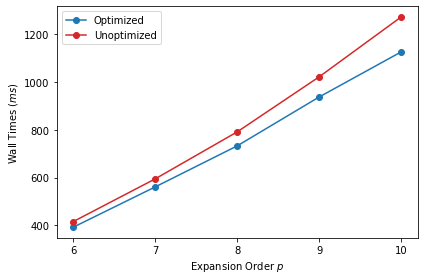
\includegraphics[width=8cm]{figures/speedup.png}}
    \caption{Minimum runtime of cache optimized L2P compared to a naive parallel iteration over leaves. Computed over seven trials over $32768$ leaves, with $n_{crit}=150$ and $p=6$.}
	\label{fig:l2p_cache}
\end{figure}


Due to their large interaction lists, this strategy too expensive in terms of memory for the near field, M2L and M2P operators. For example, allocating an array large enough to store the maximum possible number of source particle coordinates in double precision for the M2P operator; with $|W|=148$ and $n_{crit}=150$, requires $\sim 17$GB, and a runtime cost for memory allocations that exceeds the computation time. Instead, for the M2L we perform a parallel loop over the target nodes at each given level, and over the leaf nodes for the M2P and near field, looking up the relevant data from the linear tree as needed. The P2L interaction list of each target is at most 19 nodes, and the P2M must also calculate a check potential, cancelling out any speedup from cache locality for these operators.

The matrices involved in the M2M and L2L operators can be precomputed and scaled at each level \cite{Wang2021}, and their application is parallelized over all nodes at a given level.

Multithreading in this way means that we call the P2P, P2M, M2P, L2P and near field operators once during the algorithm, the M2L and L2L are called $d-2$ times, and the M2M is called $d$ times, where $d$ is the depth of the octree. This is the minimum number of calls while keeping the operator implementations separate for unit testing.

Figure (\ref{fig:cpu_wall}) compares the time spent within each Numba-compiled operator (`CPU time') to the total runtime (`wall time') of each operator. The wall time includes the time to (un)box data, organize inputs for Numba compiled functions, and pass control between Numba and Python. Except for the L2P which has a different parallelization strategy, the runtime costs are less than 5 \% of each operator's total wall time, implying that we are nearly always running multithreaded code and that the CPU is nearly fully utilized. 

 % Smaller figure
 \begin{figure}
	\centerline{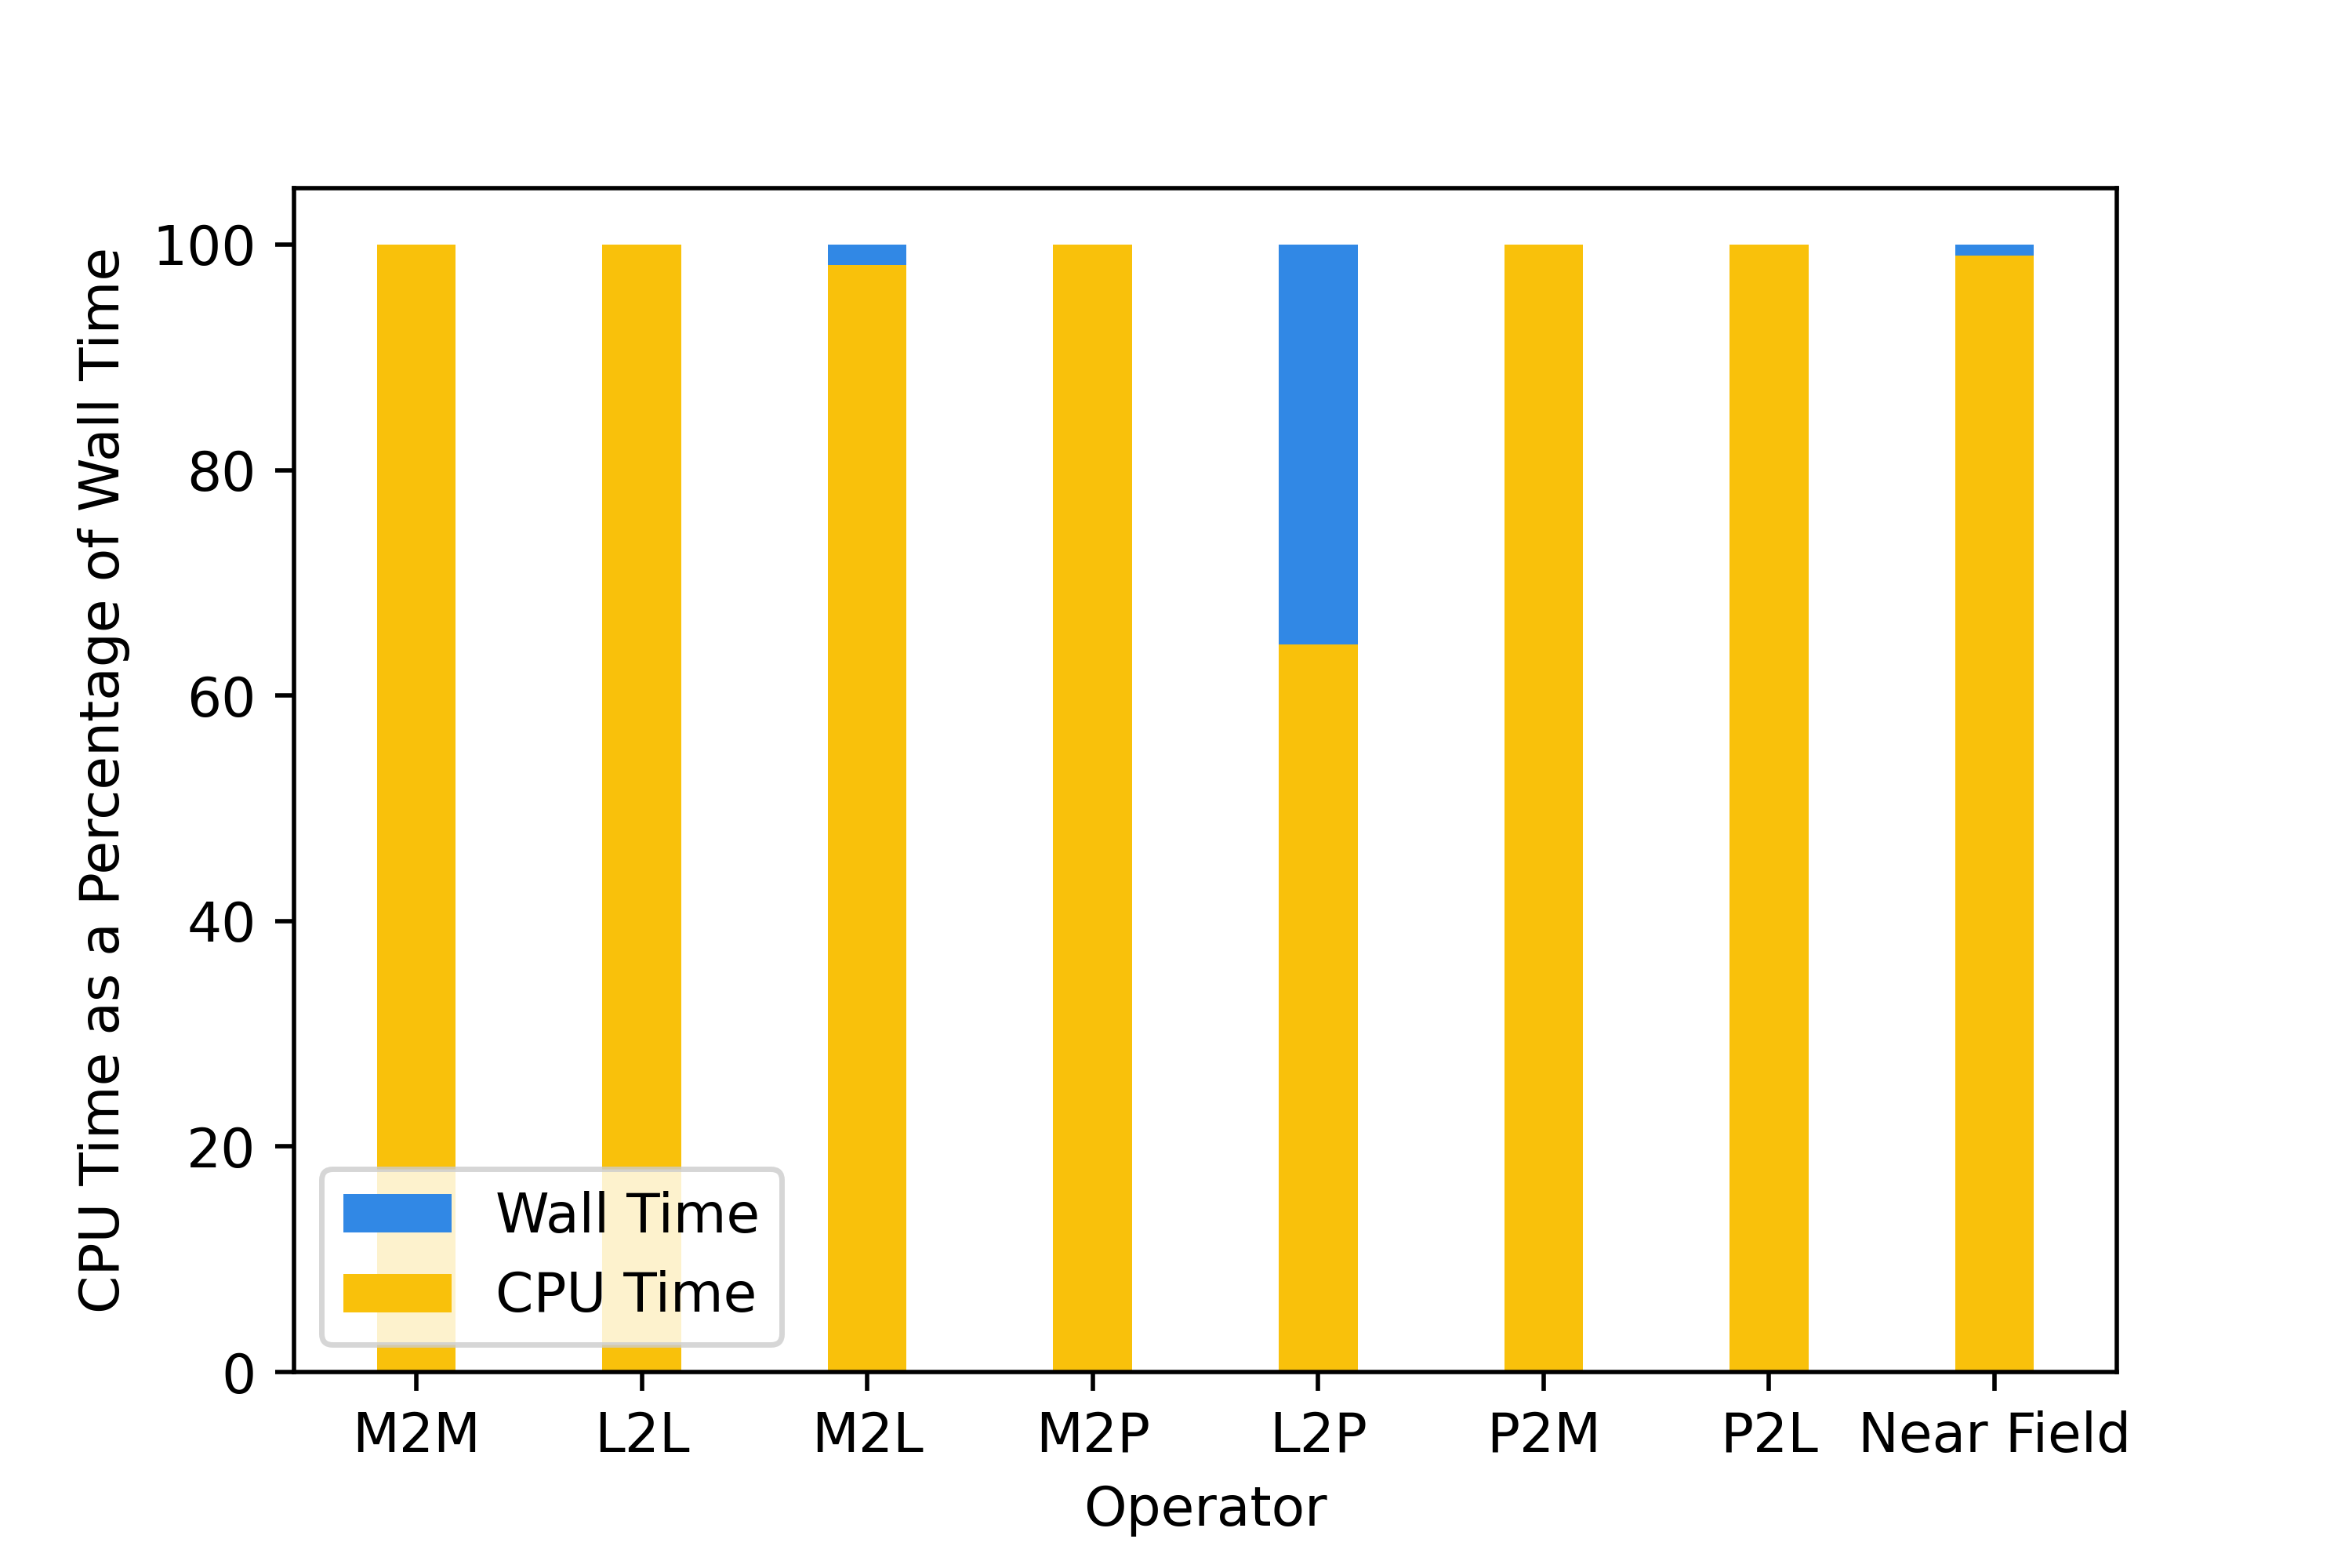
\includegraphics[width=8cm]{figures/cpu_wall.png}}
    \caption{CPU time as a Percentage of Wall time for operators. Computed over seven trials over $32768$ leaves, with $n_{crit}=150$ and $p=6$.}
	\label{fig:cpu_wall}
\end{figure}

\section{CONCLUSION}

In developing PyExaFMM we found that achieving performance with Numba is not trivial.
Achieving optimal multithreaded performance requires careful consideration of the algorithm being accelerated, details of Numba's backend implementation, as well as a design that suits Numba's data oriented framework. This is arguably more software development expertise than many in Numba's target audience can be reasonably expected to possess, making achieving performance with Numba as complex as with a compiled language. Despite this, Numba is a remarkable tool. Projects which value Python's simple cross platform builds, as well as large open source ecosystem, and only contain a small number of isolated performance bottlenecks, would benefit the most from a Numba implementation.

\section{ACKNOWLEDGMENT}

SK is sported by EPSRC Studentship 2417009.

\bibliography{pyexafmm}

\bibliographystyle{ieeetr}

\begin{IEEEbiography}{Srinath Kailasa}{\,}is a PhD student in Mathematics at University College London.
\end{IEEEbiography}

\begin{IEEEbiography}{Tingyu Wang}{\,}is a PhD student in Mechanical Engineering at the George Washington University. Contact him at twang66@email.gwu.edu.
\end{IEEEbiography}

\begin{IEEEbiography}{Lorena. A. Barba}{\,}is a Professor of Mechanical and Aerospace Engineering at the George Washington University.  Contact her at labarba@email.gwu.edu.
\end{IEEEbiography}

\begin{IEEEbiography}{Timo Betcke}{\,} is Professor of Computational Mathematics at University College London.
\end{IEEEbiography}

\end{document}

